\documentclass[10pt,twocolumn,twoside]{base/ijb}

% Article information (authors ignore)
\articleno{XX(X), XXXX, XX-XX}
\doifooter{\href{http://dx.doi.org/10.22146/ijbiotech.xxxxx}{10.22146/ijbiotech.xxxxx}} 
\submitted{1 Month 2000} \revised{1 Month 2000} \accepted{1 Month 2000}

% Article title
\title{The IJBiotech {\LaTeX} template}

% Author(s)
\author[1,$^*$]{First author}
\author[2]{Second author}
\author[2]{Third author}

\authorheader{Author et al.} % Author name(s) as they should appear in the header

% Author(s) affiliations
\affil[1]{Provide the full postal address of each author's affiliation, including the street name and number, city, ZIP code, and country.}
\affil[2]{Affiliation of the second and third authors}
% Corresponding author
\affil[$\ast$]{Corresponding author: \href{email@address.com}{email@address.com}}

% Abstract
\begin{abstract}
Place your abstract here. It should consist of a single paragraph of no more than 200 words. Provide the background and objective of the paper (including its originality), its principal results, and its conclusions. Avoid using abbreviations and citations.
\end{abstract}

% Keywords
\keywords{include a maximum of five keywords or phrases; separated by semicolons; order keywords alphabetically; use specific, relevant terms that do not appear in the title; do not use terms that are too general or too long}

% PDF metadata (authors ignore)
\makeatletter
	\hypersetup{%
		pdftitle={\@title},%
		pdfauthor={\authorheader},%
    	pdfkeywords={\@keywords},%
    }
\makeatother

\makeatletter
\def\MT@warn@unknown{}
\makeatother

\begin{document}

\setcounter{page}{1}

\maketitle
\thispagestyle{firststyle}
\linenumbers % Add line numbers

\section{Introduction}

This section should briefly explain the background of the study, provide a short review of the pertinent literature, state the originality of the research, and state the research objectives. 

\section{Materials and methods}

Combine the materials and methods used into one narrative passage. Enough information should be provided to enable repetition of the research. For commercial sources of the materials, the name of the company, and the town and country in which they are located should be indicated. Methods already published should be indicated by a reference, with only the relevant modifications described here; e.g. "Powder solubility was evaluated according to the method proposed by Smith (2000), with modifications. In the case of this study, powders were stirred in 25 mL of distilled water for 5 min using a blender."; or "The powder solubility test followed the method of Smith (2000), with modifications in water volume. Powders were stirred in 25 mL of distilled water for 5 min using a blender."

\section{Results}

Describe the outcome of the study. Data should be presented as concisely as possible, and in the form of tables or figures if appropriate, although very large tables should be avoided. If needed, this section can be combined with the Discussion section into a "Results and discussion" section.

Figure \ref{fig:1} shows an example figure.

\begin{figure}[b]
	\centering
	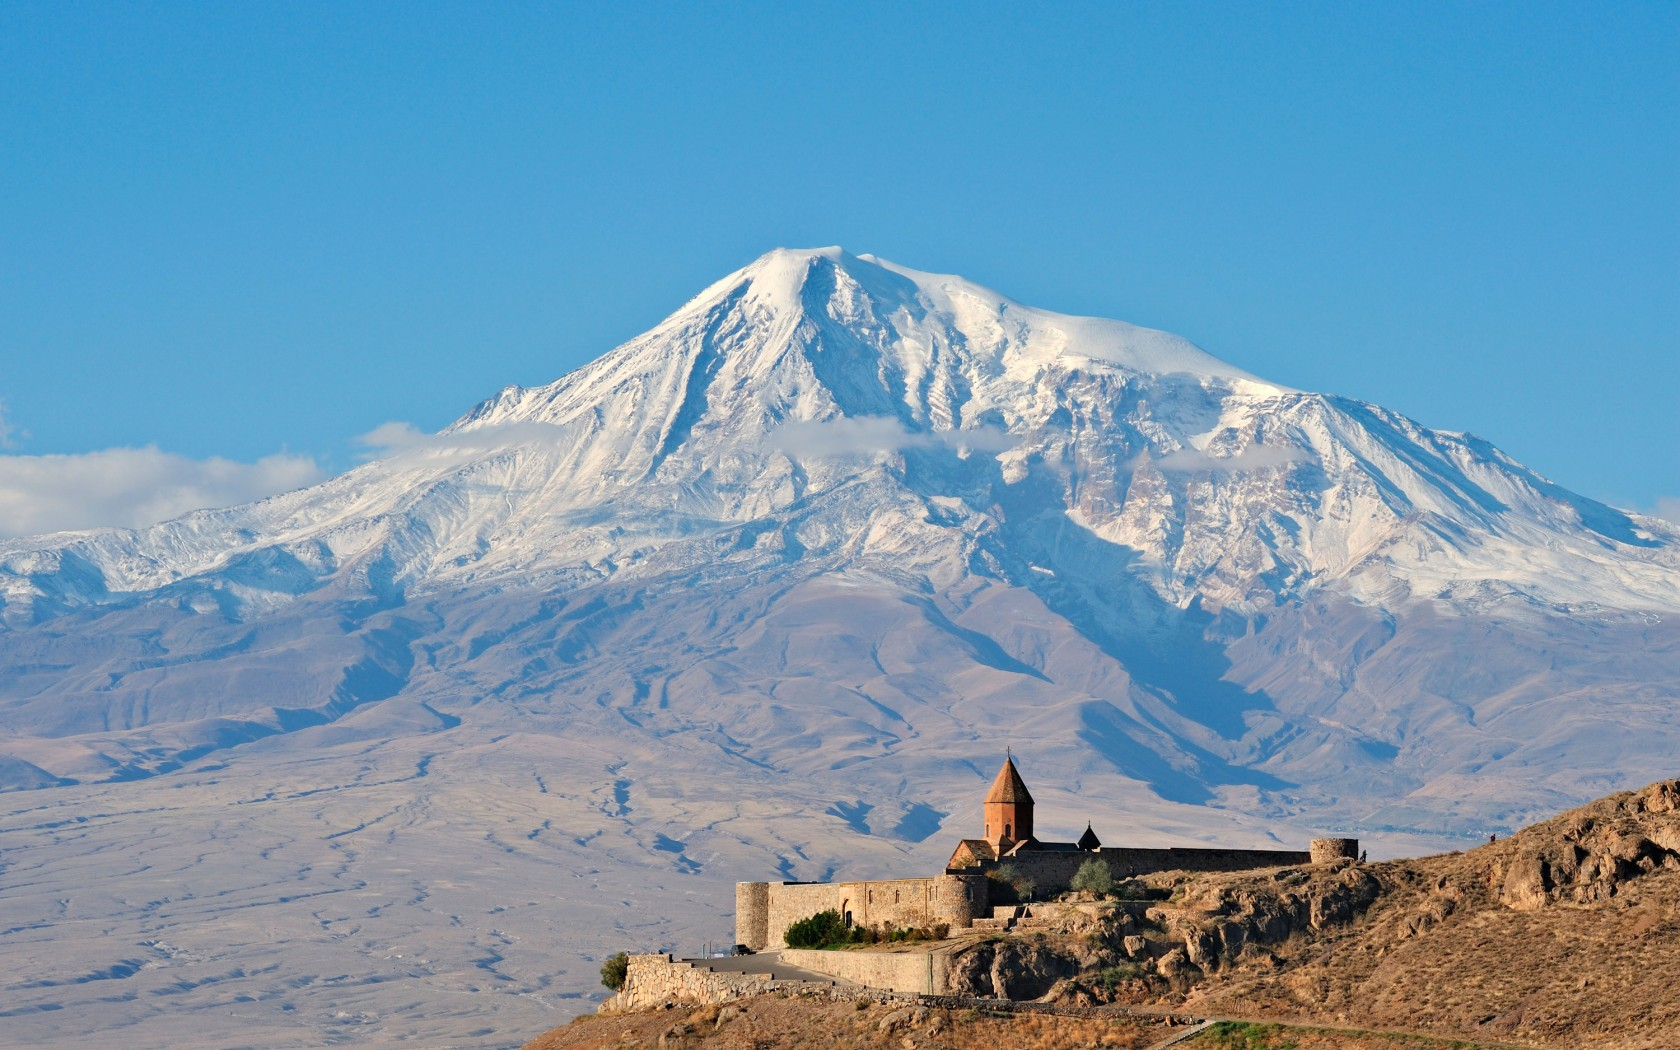
\includegraphics[width=\linewidth]{figures/example-figure}
	\caption{Example figure.}
	\label{fig:1}
\end{figure}

\begin{table}[b]
  	\centering\footnotesize\sffamily
  	\caption{This is an example table caption.}
  	\begin{tableminipage}{\linewidth}
    	\begin{tabularx}{\linewidth}{lX}
			\toprule
    		First column & Second column \\
    	  	\midrule
      		1 & This is a single-column table. To span two columns add $\ast$ to the table environment; i.e.  \verb+\begin{table*}+ and \verb+\end{table*}+ \\
      		2 & Use only horizontal lines for borders. \\
	  		\bottomrule
    	\end{tabularx}
    	\label{tab:4}
    
    	Place table footnotes here, indicating them with superscripted lowercase letters or asterisks (for significance values and other statistical data).
  	\end{tableminipage}
\end{table}




\begin{figure*}[t]
  \centering
  \captionsetup[subfigure]{justification=centering}
  \begin{subfigure}[b]{0.37\textwidth}
    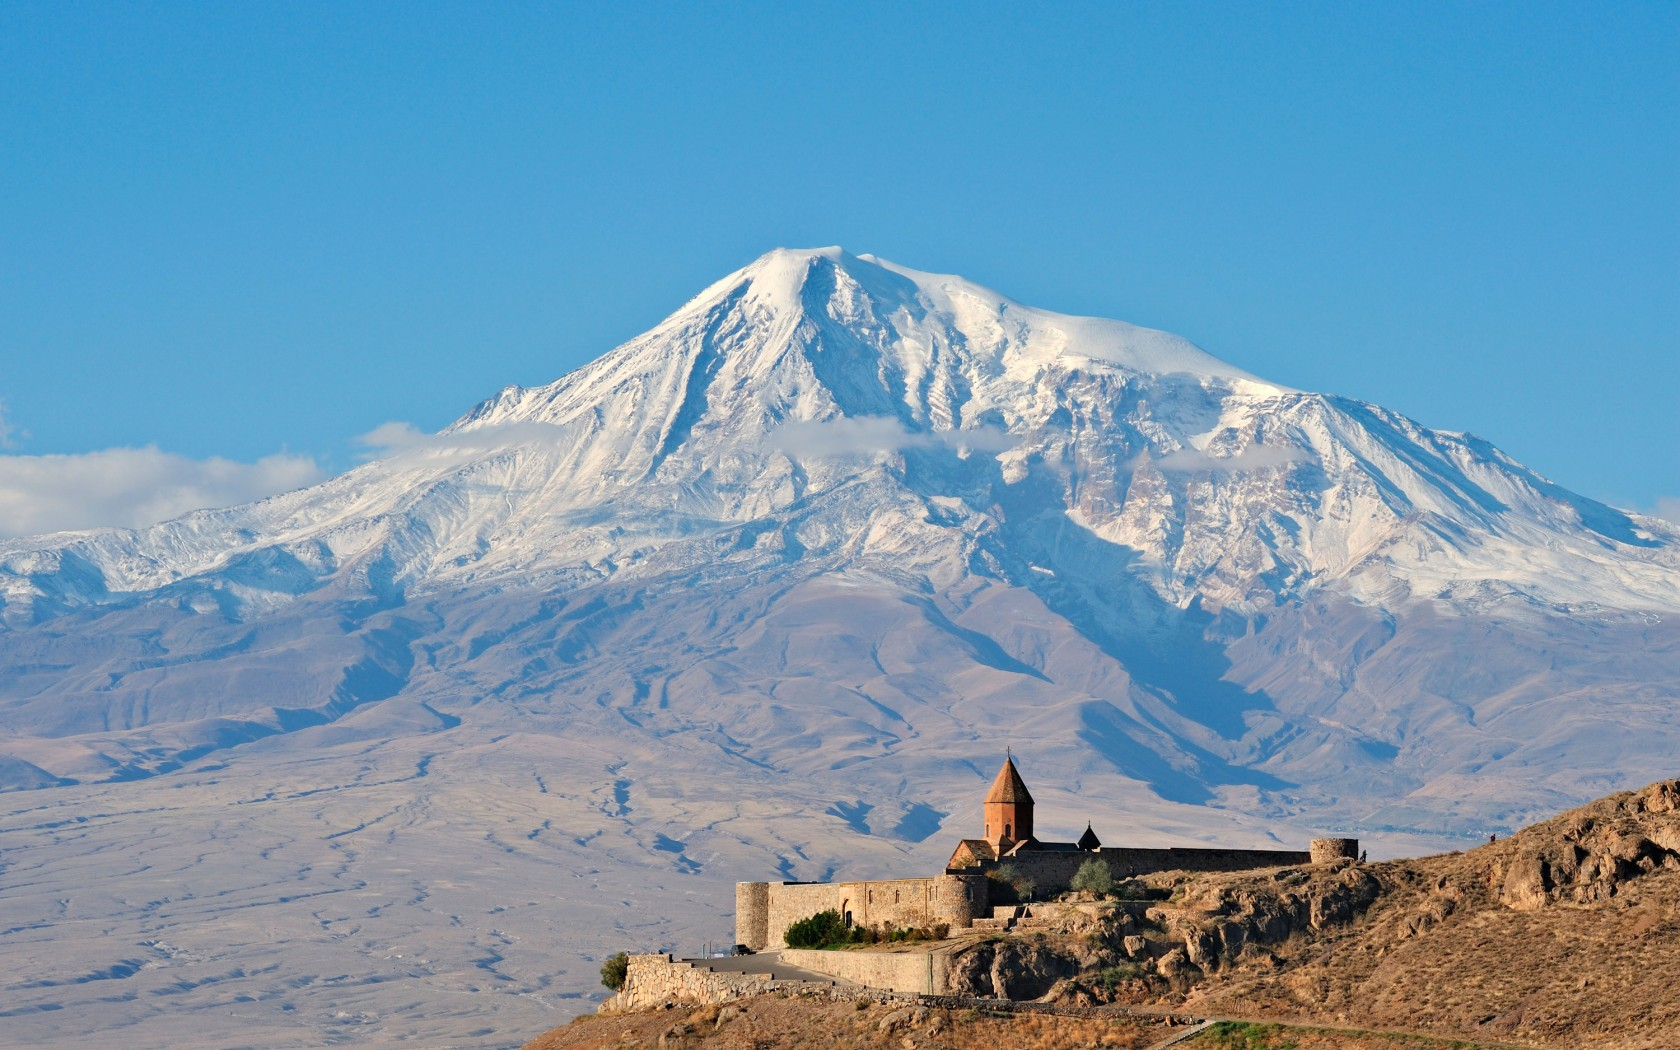
\includegraphics[width=\textwidth]{figures/example-figure}
    \caption{}
    \label{fig:1a}
  \end{subfigure}
  \qquad % Spacing between images
  \begin{subfigure}[b]{0.37\textwidth}
    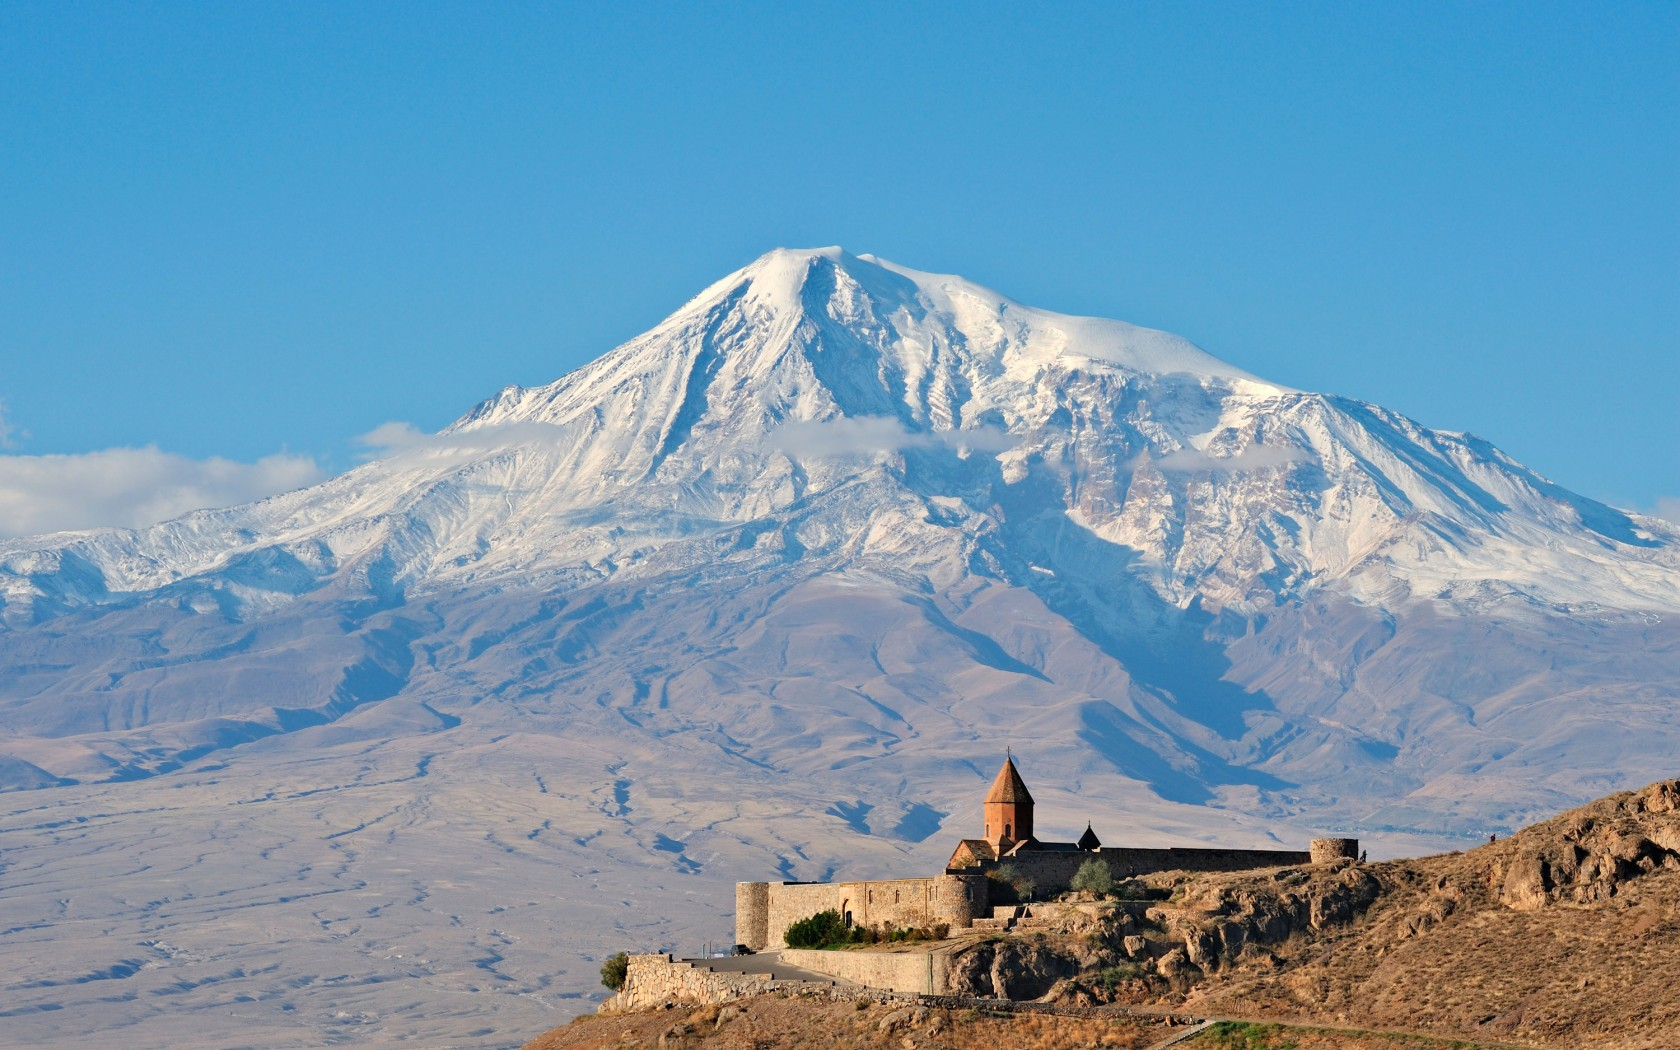
\includegraphics[width=\textwidth]{figures/example-figure}
    \caption{}
    \label{fig:1b}
  \end{subfigure}
  \caption{The RNAfold computational results of: (a) lncRNA PVT1 Human;  (b) lncRNA PVT1 \textit{Mus musculus}. Both are annotated as MFE secondary structure, the one with the most minimal free energy gibbs. The scale in the left side refers to the base pair probability, from 0 (blue) to 1 (red).}
  \label{fig:1}
\end{figure*}

\section{Discussion}

This section should be an interpretation of the results of the work (not a repetition of them) in the context of previous research. Avoid excessive referencing of published literature. If needed, this section can be combined with the Results section into a Results and discussion section.

\section{Conclusions}

The main conclusions of the study may be presented in a standalone Conclusions section or included as a subsection of the Discussion section.

\section*{Acknowledgments}

Acknowledge anyone who contributed to the research, as well as any funding or grants received in support of it. The names of funding organizations should be written in full, along with the grant numbers, if available. List any individuals who helped you during the study (e.g. assistance with study design or analysis, or guidance through a study area), or writing of the article (e.g. providing advice on the language, editing, or proofreading the article).

\section*{Authors’ contributions}

List the details of each author’s contribution to the research and manuscript. Authorship should be restricted to those who have contributed significantly to the work by either: conceiving of or designing the study, contributing new methods or models, performing research, analyzing data, or writing the paper. Use author’s initials to indicate their names; e.g. "DS, PK designed the study. DS, PK, BTF, GH carried out the laboratory work. DS, BTF, GH, MJ, DW analyzed the data. PK, BTF, GH, MJ, DW wrote the manuscript. All authors read and approved the final version of the manuscript."

\section*{Competing interests}

Declare any competing interests, such as any financial, professional, or personal relationships that are relevant to the submitted work. This can include the name of a funding source and a description of their role in the design of the study, data collection and analysis, writing of the article, and/or decision to submit the manuscript to IJBiotech; whether they serve or have previously served on IJBiotech’s editorial board; and/or whether they work or have worked for an organization that may benefit from the publication of the article.

\section{In-text Citations}

Add citations using the \verb|\citep{}| command, for example \citep{neher2013genealogies} or for multiple citations, \citep{neher2013genealogies, rodelsperger2014characterization}

\section{Examples of Article Components}
\label{sec:examples}

The sections below show examples of different header levels, which you can use in the primary sections of the manuscript (Results, Discussion, etc.) to organize your content.

\section{Sample Equation}

Let $X_1, X_2, \ldots, X_n$ be a sequence of independent and identically distributed random variables with $\text{E}[X_i] = \mu$ and $\text{Var}[X_i] = \sigma^2 < \infty$, and let
\begin{equation}
S_n = \frac{X_1 + X_2 + \cdots + X_n}{n}
      = \frac{1}{n}\sum_{i}^{n} X_i
\label{eq:refname1}
\end{equation}
denote their mean. Then as $n$ approaches infinity, the random variables $\sqrt{n}(S_n - \mu)$ converge in distribution to a normal $\mathcal{N}(0, \sigma^2)$.

\section*{References}

For the purposes of efficiency and conciseness, avoid using more than 25 references and less than 10. IJBiotech uses an author-date citation system based on The Council of Science Editors' (CSE) Scientific Style and Format. Authors can download the IJBiotech citation guide from its website, which provides common examples of how to cite and format references. For more comprehensive instructions, refer to CSE's Scientific Style and Format (8th edition). For references in a non-English language, provide the English translation between square brackets ([ ]) right after the title. Authors are strongly urged to use a reference manager such as Zotero or Mendeley to build their bibliography, saving the file in .bib format.

Below is an example of what your reference list should look like.

\bibliography{references}
\atColsEnd{\vfill}

\end{document}